\documentclass[11pt, a4paper, twoside, openright, openany]{book} %draft

\usepackage{graphicx,color}
\usepackage{amssymb, amsmath, array}
\usepackage{cite}
\usepackage[T1]{fontenc}

\usepackage{listings}
\usepackage{color}
\usepackage{dirtytalk}
\usepackage{url}

\graphicspath{{illustrations/}}

\begin{document}

% Example of title page for the projects carried out within DEDIS
% Copied from lasec

% Simply include it in your mastex tex file:
%        % Example of title page for the projects carried out within DEDIS
% Copied from lasec

% Simply include it in your mastex tex file:
%        % Example of title page for the projects carried out within DEDIS
% Copied from lasec

% Simply include it in your mastex tex file:
%        \input{cover}


% Updated October 2016


\newcommand{\logoepfl}[0]{
  \begin{center}
    
\includegraphics[width=4cm]{logo_epfl_coul.eps}
  \end{center}
  \vspace{0.3cm}
  \hrule
}
\newcommand{\project}[1]{
  \begin{center}
    \large{#1}
  \end{center}
  \vspace{1cm}
}
\newcommand{\department}[1]{
  \begin{center}
    \large{#1}
  \end{center}
}
\newcommand{\lab}[1]{
  \begin{center}
    \large{#1}
  \end{center}
}
\newcommand{\supervisor}[3]{
  \begin{center}
    \begin{normalsize}{
        \bf #1}\\#2\\#3
    \end{normalsize}
  \end{center}
}
\renewcommand{\author}[1]{
  \begin{center}
    \Large{#1}
  \end{center}
  \vspace{0.5cm}
}
\renewcommand{\title}[1]{
  \vspace{3cm}
  \begin{center}
    \huge{#1}
  \end{center}
  \vspace{1.7cm}
}
\renewcommand{\date}[2]{
  \begin{center}
    \normalsize{#1 #2}
  \end{center}
  \vspace{0.5cm}
}


\thispagestyle{empty}


% begin title page
  \logoepfl
  
  \title{Web-Frontend for Cothority}

  \author{Bastian Nanchen}
  \department{School of Computer and Communication Sciences}
  \lab{Decentralized and Distributed Systems lab}
  \project{Semester Project}

  \date{December}{2016}

  \begin{center}
    \begin{tabular}{cc}
      \begin{tabular}{p{4.0cm}}
        \supervisor{Responsible}{Prof.Bryan Ford}{EPFL / DEDIS}
      \end{tabular}&
      \begin{tabular}{p{4.0cm}}
        \supervisor{Supervisor}{Linus Gasser}{EPFL / DEDIS}
      \end{tabular}
    \end{tabular}
  \end{center}

% end title page



% Updated October 2016


\newcommand{\logoepfl}[0]{
  \begin{center}
    
\includegraphics[width=4cm]{logo_epfl_coul.eps}
  \end{center}
  \vspace{0.3cm}
  \hrule
}
\newcommand{\project}[1]{
  \begin{center}
    \large{#1}
  \end{center}
  \vspace{1cm}
}
\newcommand{\department}[1]{
  \begin{center}
    \large{#1}
  \end{center}
}
\newcommand{\lab}[1]{
  \begin{center}
    \large{#1}
  \end{center}
}
\newcommand{\supervisor}[3]{
  \begin{center}
    \begin{normalsize}{
        \bf #1}\\#2\\#3
    \end{normalsize}
  \end{center}
}
\renewcommand{\author}[1]{
  \begin{center}
    \Large{#1}
  \end{center}
  \vspace{0.5cm}
}
\renewcommand{\title}[1]{
  \vspace{3cm}
  \begin{center}
    \huge{#1}
  \end{center}
  \vspace{1.7cm}
}
\renewcommand{\date}[2]{
  \begin{center}
    \normalsize{#1 #2}
  \end{center}
  \vspace{0.5cm}
}


\thispagestyle{empty}


% begin title page
  \logoepfl
  
  \title{Web-Frontend for Cothority}

  \author{Bastian Nanchen}
  \department{School of Computer and Communication Sciences}
  \lab{Decentralized and Distributed Systems lab}
  \project{Semester Project}

  \date{December}{2016}

  \begin{center}
    \begin{tabular}{cc}
      \begin{tabular}{p{4.0cm}}
        \supervisor{Responsible}{Prof.Bryan Ford}{EPFL / DEDIS}
      \end{tabular}&
      \begin{tabular}{p{4.0cm}}
        \supervisor{Supervisor}{Linus Gasser}{EPFL / DEDIS}
      \end{tabular}
    \end{tabular}
  \end{center}

% end title page



% Updated October 2016


\newcommand{\logoepfl}[0]{
  \begin{center}
    
\includegraphics[width=4cm]{logo_epfl_coul.eps}
  \end{center}
  \vspace{0.3cm}
  \hrule
}
\newcommand{\project}[1]{
  \begin{center}
    \large{#1}
  \end{center}
  \vspace{1cm}
}
\newcommand{\department}[1]{
  \begin{center}
    \large{#1}
  \end{center}
}
\newcommand{\lab}[1]{
  \begin{center}
    \large{#1}
  \end{center}
}
\newcommand{\supervisor}[3]{
  \begin{center}
    \begin{normalsize}{
        \bf #1}\\#2\\#3
    \end{normalsize}
  \end{center}
}
\renewcommand{\author}[1]{
  \begin{center}
    \Large{#1}
  \end{center}
  \vspace{0.5cm}
}
\renewcommand{\title}[1]{
  \vspace{3cm}
  \begin{center}
    \huge{#1}
  \end{center}
  \vspace{1.7cm}
}
\renewcommand{\date}[2]{
  \begin{center}
    \normalsize{#1 #2}
  \end{center}
  \vspace{0.5cm}
}


\thispagestyle{empty}


% begin title page
  \logoepfl
  
  \title{Web-Frontend for Cothority}

  \author{Bastian Nanchen}
  \department{School of Computer and Communication Sciences}
  \lab{Decentralized and Distributed Systems lab}
  \project{Semester Project}

  \date{December}{2016}

  \begin{center}
    \begin{tabular}{cc}
      \begin{tabular}{p{4.0cm}}
        \supervisor{Responsible}{Prof.Bryan Ford}{EPFL / DEDIS}
      \end{tabular}&
      \begin{tabular}{p{4.0cm}}
        \supervisor{Supervisor}{Linus Gasser}{EPFL / DEDIS}
      \end{tabular}
    \end{tabular}
  \end{center}

% end title page


\begingroup
\let\cleardoublepage\clearpage
\tableofcontents
\endgroup


\chapter{Introduction}
Distributed cryptography spreads the operation of a cryptosystem among a group
of servers in a fault-tolerant way~\cite{definition}.
\newline
The DeDis team at EPFL is working among others on a software project called \say{Cothority}.
Cothority (Decentralized Withness Cosigning) is a \say{multi-party cryptographic signatures}~\cite{cothorityInfo}.
\newline
In order to accomplish that they developed the CoSi protocol (Collective Signing),
which will produce a collective signature by decentralized servers.
The outcoming signature has the same verification cost and size as an individual signature.
A digital signature is used to verify a file's origin and content.
\newline
This endeavor addresses a significant issue. Per example a certificate or a software
update now needs one single signature from a corporate or a government (or anything/anybody) to validate it.
This represents a high-value item for criminals, intelligence agency,\ldots
The CoSi protocol provides a validation at every authoritative statement a validation,
which is produced by a group of independent parties (named conodes),
before any device or client use it~\cite{cosi}.\\


% TODO:presentation of the report!!!!!!!!!!!!!!!!!!!!!!!!!!!!!!!!!

\chapter{Aims and goals}
The goal of this semester project is to furnish a web-interface to the Cothority project.
\newline
The aims stated are to provide a status-array with informations like port number,
name or bandwidth used for each contacted conodes, to be able to send a file for
a digital signature using the CoSi protocol and to verify if a digital signature
corresponds to a particular file.\\

\chapter{Tools utilised}
Obviously the language choosen to implement the web-interface is JavaScript.
The HTML markup language and the CSS style sheet language are used as well.
\newline
The Bootstrap framework~\cite{bootstrap} is employed for designing the website.\\

\section{Libraries}
Several libraries are used in the semester project.
\newline
The jQuery library~\cite{query} is utilized to
facilitate the selection and modification of DOM (Document Object Model) elements.\\

The protobuf.js~\cite{protobufjs} is a pure JavaScript implementation of Google's Protobuf.
It uses the same format of .proto file.
The Cothority's approach for serializing structured data is a Google's Protobuf-like.
It seems evident to use the same way for the web-interface.
\newline
\say{Protocol buffers are a flexible, efficient, automated mechanism for
serializing structured data-think XML, but smaller, faster, and simpler.}~\cite{protobufDefi}.\\

\begin{lstlisting}[caption={Example of .proto file}, captionpos=b]
 message Foo{
            required bytes a = 1;
            optional bytes b = 2;
        }
\end{lstlisting}
\leavevmode \\

A .proto file is composed of protocol buffer message(s). Each message contains name-value pair(s).
The value is a unique tag. Each tag is \say{used to identify your
 fields in the message binary format}~\cite{protobufDefi}.
Each pair has a type. There is multiple disponible tags.
\newline
The last element to define is rule field. The web-interface
uses two rule fields: \say{required} and \say{optional}. The protocol buffer message
with a \say{required} field is obligate to send or receive the field, contrary to
the message with a \say{optional} field, which is not obligate to send or receive the field in question.\\

The js-nacl~\cite{jsnacl} library is adopted in the Verification part of the project.
As said on the library's GitHub page: \say{A high-level Javascript API wrapping an Emscripten-compiled libsodium, a cryptographic library based on NaCl. Includes both in-browser and node.js support.}.
NaCl (Networking and Cryptography library) is a software library written in C for
network communication, encryption, decryption, signatures,\ldots~\cite{nacl}. Its
goal is to \say{provide all of the core operations needed to build higher-level cryptographic tools}~\cite{nacl}.
Little disclaimer NaCl is pronounced \say{salt}.\\

Other libraries like js-nacl, protobuf.js,etc.\ are used and will be presented
in subsections below.\\

\chapter{Problems that arose and solutions implemented to solve them}
\section{Status Part}
The first problem to tackle was the create a communication between the website
and a conode.
\newline
The object Websocket~\cite{websocketPage} of the JavaScript Web APIs offers the tools to create a communication
between a browser and a server and send/receive data.
\newline
At first an empty protocol buffer message is sent in a Blob~\cite{blob} object containing
the .proto file in bytes.\\

\begin{lstlisting}[caption={Empty protocol buffer message}, captionpos=b]
  message Request {
  }
\end{lstlisting}

The request being sent, through a Websocket object, the web page waits for response from the conode.\\

\begin{lstlisting}[caption={response protocol buffer message}, captionpos=b]
  message ServerIdentity{
    				required bytes public = 1;
    				required bytes id = 2;
    				required string address = 3;
    				required string description = 4;
				}

  message Response {
    				map<string, Status> system = 1;
    				optional ServerIdentity server = 2;

				    message Status {
        				map<string, string> field = 1;
    				}
				}
\end{lstlisting}
\leavevmode \\

The response is is a map with field corresponding to another message format, which
is a map of a string with a string. Each key corresponding to an element of the conode's
status (port number, hostname, number of bytes received and sent, number of services,
 connexion type, uptime, name and version) and each field to its value.\\

 % TODO resté ici

\section{Verification Part}


\chapter{Strategical choices undertaken during implementation}
\chapter{Results}
\chapter{Theortical and practical limitations of the project and its implementation}
\chapter{Future work}
\chapter{Theoritical and practical knowledge gained through the project}
\chapter{Step-by-step}

\iffalse
\chapter{Analysis}
The first part of the semester project was to acquire knowledge in JavaScript and
HTML and become familiar with the JQuery library. For delivering a skeleton of
the website before the beginning of the semester.\\
Next thing to settle was the communication between the website and a conode.
The JavaScript Web APIs contain all the necessary to handle this problem.
The object Websocket~\cite{websocketPage} offers all the tools to create a
communication between a browser and a server.\\

%talk about the implementation of the Status Part
\section{Status part}
The JavaScript Web APIs contain all the necessary to handle the communication
part. The object Websocket~\cite{websocketPage} offers all the tools to create a
communication between a browser and a server and send/receive data. All the elements send to conodes are .proto files.\\
First it is necessary to establish the connection. A connection is established
with each conode.\\
An empty .proto file is send in a Blob object containing the .proto file in bytes.\\

\begin{lstlisting}[caption={empty .proto file}, captionpos=b]
  message Request {
  }
\end{lstlisting}

\fi

The request being sent the webpage waits for a response. The response will be the
status of the concerning conode. It is received as a .proto file.

\begin{lstlisting}[caption={response .proto file}, captionpos=b]
  message ServerIdentity{
    				required bytes public = 1;
    				required bytes id = 2;
    				required string address = 3;
    				required string description = 4;
				}

  message Response {
    				map<string, Status> system = 1;
    				optional ServerIdentity server = 2;

				    message Status {
        				map<string, string> field = 1;
    				}
				}
\end{lstlisting}

The response is is a map with field corresponding to another message format, which
is a map of a string with a string. Each key corresponding to an element of the conode's
status (port number, hostname, number of bytes received and sent,\ldots) and each field
to its value.\\
%Mettre une subsection?????????????
\subsection{Promise API}
That being said, the response message is triggered by our opening socket message. Therefore the
response message will be asynchronous.\\
To tackle the asynchronous problem, the introduction of the Promise object in JavaScript must be
made. First it is important to know that JavaScript is single threaded. It means
that if a code snippet is waiting on data, the thread can't be waiting on it and doesn't execute
the remaining part of the code. In that case JavaScript program would be very slow.
So through the history of JavaScript many tools were created to handle asynchronous programs.
Like callback functions that was widely used, but widely disliked too. It even has a nickname:\say{Callback Hell}.\\

\begin{lstlisting}[caption={Example of Callback Hell with its typical pyramid shape}, captionpos=b]
  fs.readdir(source, function (err, files) {
  if (err) {
    console.log('Error finding files: ' + err)
  } else {
    files.forEach(function (filename, fileIndex) {
      console.log(filename)
      gm(source + filename).size(function (err, values) {
        if (err) {
          console.log('Error identifying file size: ' + err)
        } else {
          console.log(filename + ' : ' + values)
          aspect = (values.width / values.height)
          widths.forEach(function (width, widthIndex) {
            height = Math.round(width / aspect)
            console.log('resizing ' + filename + 'to ' + height + 'x' + height)
            this.resize(width, height).write(dest + 'w' + width + '_' + filename, function(err) {
              if (err) console.log('Error writing file: ' + err)
            })
          }.bind(this))
        }
      })
    })
  }
})
\end{lstlisting}
\leavevmode \\
Other libraries (jQuery) begun implementing promises to help developers overcome the \say{Callback Hell}.
This eventually leads ECMAScript 6 to adopt The Promise API~\cite{promise} natively in JavaScript~\cite{ecmaPromise}.
The object Promise allows to retrieve a value in the \say{future}.
\\
\begin{lstlisting}[caption={Structure of a Promise}, captionpos=b]
  var promise = new Promise(function(resolve, reject) {
    // asynchronous snippet code
    if (/*everything goes well*/) {
      resolve(/*result of async element*/);
    } else {
      reject(/*result of async part*/);
    }
  });
\end{lstlisting}
\leavevmode \\
A callback function needs to be passed at the Promise's constructor. This function
will have two parameters. The resolve function will be called if everything worked in
the asynchronous part, otherwise the reject function will be called.\\
In the case of this semester project, the resolve function will return the response
.proto file containing all the status data from the conode.\\

\leavevmode \\

\subsection{Generator}
To handle the Promise returned the project will use another feature of ECMAScript 6 called a Generator.
It's a new kind of function. It can be paused in the middle and resumed later. Of course,
other parts of the code are running during the pause.\\

\begin{lstlisting}[caption={Structure of a generator function}, captionpos=b]
  function* foo() {
    var x = yield 1;
  }
  \end{lstlisting}
\leavevmode \\
The \say{*} marks the function as a generator one. The other different element of
the code snippet is the keyword:\say{yield}. \say{yield \underline{\hspace{1cm}} is called a \say{yield expression} (and not a statement) because when we restart the generator, we will send a value back in, and whatever we send in will be the computed result of that yield \underline{\hspace{3cm}} expression.}
~\cite{yieldExpression}. The function will stop when it encounters the \say{yield} keyword.
Whenever (if ever) the generator is restarted, the \say{yield 1} expression will send \say{1} back.
The part following the \say{yield} keyword is the expression that will be returned.\\

 \begin{lstlisting}[caption={Restart of a generator function}, captionpos=b]
   var a = foo();
   a.next();
 \end{lstlisting}
 \leavevmode \\
The call to the \say{next()} method will execute the generator (from the last \say{yield}) to the next encounter of a \say{keyword} (if there is any).\\
Returning to the project's code, a generator function is used with the function returning a Promise object.\\

\begin{lstlisting}[caption={Extract from the project's code}, captionpos=b]
  function* generator() {
        // some code
        var message = yield websocket_status(7003);
        listNodes.push(nodeCreation(message));
        // some code
    });
}
\end{lstlisting}
\leavevmode \\
The function \say{websocket\_status()} returns a Promise object. The generator function
stops when reaching \say{websocket\_status()}. \say{The main strength of generators is that they provide a single-threaded, synchronous-looking code style, while allowing you to hide the asynchronicity away as an implementation detail.}~\cite{runGenerator}.
The idea is to \say{yield} out promises and let them restart the generator function when
they are fulfilled. To do so we need to create a new function that will control the generator function's iterator.\\
\begin{lstlisting}[caption={Extract from the project's code~\cite{runGenerator}}, captionpos=b]
  function runGenerator(g) {
    let iterator = g();
    (function iterate(message) {
        let ret = iterator.next(message);

        if (!ret.done) {
            ret.value.then(iterate);
        }
    })();
  }
\end{lstlisting}
\leavevmode \\
This function takes a generator function as parameter. The \say{iterator} function
is the generator function. The inner-function \say{iterate()} will look if a promise
returns the value \say{message} from \say{iterator.next(message)}. If not (\say{ret.done} == false), the function
will iterate again.\\

\subsection{Implementation}
Now all the elements needed are presented, it only remains to do it for each node.\\

\begin{lstlisting}[caption={Extract from the project's code reaching conodes at port 7003, 7005 and 7007}, captionpos=b]
  runGenerator(function* generator() {
        listNodes = [];
        let message = yield websocket_status(7003);
        listNodes.push(nodeCreation(message));
        message = yield websocket_status(7005);
        listNodes.push(nodeCreation(message));
        message = yield  websocket_status(7007);
        listNodes.push(nodeCreation(message));
        // some code
    });
\end{lstlisting}
\leavevmode \\
As said above the \say{websocket\_status()} function returns a Promise object. Thus
the generator function \say{generator()} will \say{yield} before each \say{websocket\_status()} call.
The generator function is given in parameter to the \say{runGenerator()} function.\\
The Promise API, the generator function and the util function \say{runGenerator()} allow to hide
the asynchronous part of the code. It is more readable and more modular.\\

% Google Chrome with async

% Not final part if recursive method done [BEGIN]
Then it only remains to do it for each node.
% Not final part if recursive method done [END]

\section{Signature part}
The semester project must implement the possibility to send a file for a collective signature
and to verify a signature.


In the Cothority project the signature is a Schnorr signature, which is a zero-knowledge proof presented
by Mr.Schnorr in 1989. It is \say{based on the intractability of certain discrete logarithm problems}~\cite{wikiSchnorr}.\\
In the part where the user can send a file and sign it by the conodes,
the website needs to calculate the aggregate-key using the public-keys of the conodes.
More details will be presented in the Implementation subsection.\\
The private and the public-key used in the Cothority project require the usage of
the Edwards-curve Digital Signature Algorithm (edDSA).
\say{edDSA is a variant of Schnorr's signature system with Twisted Edwards curves.}~\cite{edDSA}.
The Cothority project uses Ed25519, which is an instantiation of EdDSA, for the
public-key signature. Ed25519 has some interesting aspect as a fast key generation,
small keys and an high security level~\cite{ed25519}.\\
% TODO deplace the above paragraph?!?!?!

The user has the possibility to submit a file and download a JSON file with the
signature and other informations.\\

\subsection{Send a file for a collective signature}

\subsubsection{Analysis}
The calculation of the aggregate-key shall be done in the website for security reason.
The server could make up a pair of public and private-keys, sign with it and send
the make up public-key to the website as the aggregate-key. The security of all
the servers would be questioning.
To accomplish it the program needs to collect the public-key of each servers.
Then given that the Cothority project uses Ed25519 % TODO ici suite à écrire!

\subsubsection{Implementation}
The implementation of the HTML part is straightforward. It needs an input tag to
submit a file and all the collapse-thing is managed by the Bootstrap framework~\cite{bootstrap}.\\

\begin{figure}[ht!]
\centering
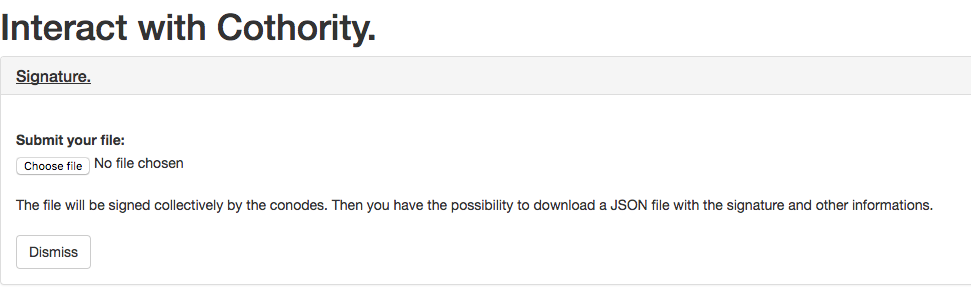
\includegraphics[width=125mm]{verification_signature.jpg}
\caption{Interface}
\end{figure}
\leavevmode \\

The file submitted is read as an ArrayBuffer~\cite{ArrayBuffer}. The Promise APIs,
a generator function and the \say{runGenerator()} function are used to deal with
the asynchronous part of submitting a file. The reading of the file is returned
inner a Promise object in a generator function that is given in paramter to the
\say{runGenerator()} util function (go to subsection n°2.1 for more details on
the manner to tackle the asynchronous part).\\ % TODO come back for the number of the subsection

% TODO déplacer ce paragraphe en haut?!?!
Afterward the file needs to be signed. To do so the program uses two libraries
protobuf.js~\cite{protobufjs} that was introduced before and js-nacl~\cite{jsnacl}.
As said on the library's GitHub page: \say{A high-level Javascript API wrapping an Emscripten-compiled libsodium, a cryptographic library based on NaCl. Includes both in-browser and node.js support.}.
NaCl (Networking and Cryptography library) is a software library written in C for
network communication, encryption, decryption, signatures,\ldots~\cite{nacl}. Its
goal is to \say{provide all of the core operations needed to build higher-level cryptographic tools}~\cite{nacl}.
Little disclaimer NaCl is pronounced \say{salt}.\\
In this semester project the js-nacl library is employed to generate a SHA-256 of the file and
to verify the signature knowing the hash of the file and the aggregate-key.\\

When the websocket is appropriately opened, the communication is done through a websocket
using 4 \.proto file messages.

\begin{lstlisting}[caption={.proto file}, captionpos=b]
  message ServerIdentity{
            required bytes public = 1;
            required bytes id = 2;
            required string address = 3;
            required string description = 4;
        }

        message Roster {
            optional bytes id = 1;
            repeated ServerIdentity list = 2;
            optional bytes aggregate = 3;
        }

        message SignatureRequest {
            required bytes message = 1;
            required Roster roster = 2;
        }

        message SignatureResponse {
            required bytes hash = 1;
            required bytes signature = 2;
            required bytes aggregate = 3;
        }
\end{lstlisting}
\leavevmode \\

As said in the Analysis subsection the website needs to calculate the aggregate-key.
Initially a list of each conode's public-key needs to be created. The status part
of the website looks after collecting servers' informations every 3 seconds. A variable,
which contains all the informations of the conodes, is added to the \say{window} object.
Adding an element to the \say{window} object is a proper way to define a global variable
in JavaScript~\cite{globalVariable}. Thus this list is used to collect each public-key
of the conodes. Having that the calculation of the aggregate-key can begin.
The program utilizes an other NaCl library: \say{TweetNaCl.js}~\cite{tweetNacl} to
pack and unpack %* TODO what?!?
and to addition the points.\\

\begin{lstlisting}[caption={Extract of the code calculating the aggregate-key}, captionpos=b]
  const listServers = window.listNodes.map(function(node, index) {
                const server = node.server;
                const pub = new Uint8Array(server.public.toArrayBuffer()); // public key of a server
                // the point is represented as a 2-dimensional array
                const pubNeg = [gf(), gf(), gf(), gf()]; // zero-point
                unpackneg(pubNeg, pub);
                const pubPosArr = new Uint8Array(32);
                pack(pubPosArr, pubNeg);
                const pubPos = [gf(), gf(), gf(), gf()]; // zero-point
                unpackneg(pubPos, pubPosArr);
                if (index == 0) {
                    agg = pubPos;
                } else {
                    // add pubPos to agg, storing result in agg
                    add(agg, pubPos);
                }
                return new siProto({public: server.public, id: server.id, address: server.address,
                    description: server.description});
            });
            pack(aggKey, agg);
\end{lstlisting}
\leavevmode \\

Having calculated the aggregate-key, the website sends to one conode the list of servers
and the hash of the file. The server responds with a message containing the signature
and the hash of the file. The server's response and the aggregate-key are entrusted to a function \say{saveToFile(fileSigned, filename, message)}.
The function takes as parameters the signed file contained inside an ArrayBuffer,
the filename and an array message containing the signature and the aggregate-key.
The function calculates the SHA-256 hash of the file using a function from js-nacl library.
The signature, the aggregate-key and the hash are translated in base64 to be more readable.\\

From there on the JSON file is created and proposed to be downloaded to the website's user.
The JSON file contains the signature's file, the filename, the date, the aggregate-key and the file's hash.\\

\begin{lstlisting}[caption={Example a downloadable JSON file}, captionpos=b]
  "filename": "file",
  "date": "3/12/2016",
  "signature": "vVppwEgya0T22mGlKBfj4Tx+BVQQx0EAH3XFLClfwSbskCxEsPIJ62ZUoD3N7ksRCEK2M/XA6flV2tLsiQmrAf4=",
  "aggregate-key": "IjgFxLpeV8IOVShIGC6ESh4cnczF1m5RRSE8jguueG4=",
  "hash": "9UmFDLT4jzzfTMZv/5O71Bh73KTlrOTQXKgKYNC/Z0Y="
\end{lstlisting}
\leavevmode \\

The JSON file is downloadable using a Blob object~\cite{blob}.

\subsection{Verification}

\subsubsection{Analysis}
The user needs to submit a JSON file in the same form as the JSON file downloadable
as previously said. The website have the ability to verify two things.
First if the hash of the file is the same as the hash on the JSON file. Second if the signature
is correct.\\
To accomplish the first part, the program extracts the hash from the JSON file and
calculates the SHA-256 hash of the submitted file and compare the two of them.\\
The second part, % TODO partie obscure de comment la librairie vérifie cela. Le code sur GitHub est illible

\subsubsection{Implementation}
The UI section is completed following the same behavior as before.\\

\begin{figure}[ht!]
\centering
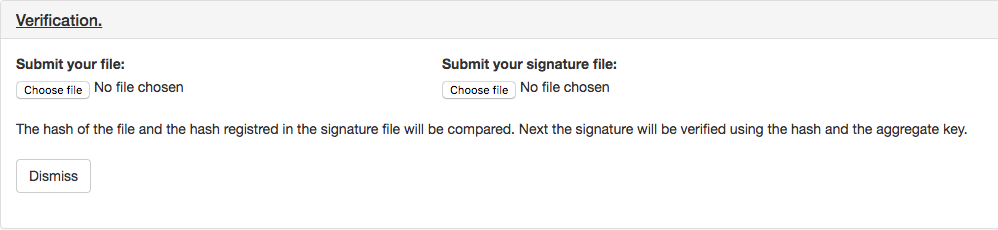
\includegraphics[width=125mm]{verification_verification.jpg}
\caption{Interface}
\end{figure}
\leavevmode \\

The submit of the two files is done in the same way as in the \say{Send a file for a collective signature} part
using Promise APIs, a generator function and \say{runGenerator()} function.
The program translates the JSON file into an object due to the native function \say{JSON.parse()}.\\
The program calculates the SHA-256 hash of the submitted file using the same method as in the
subsection: \say{Send a file for a collective signature} from the js-nacl~\cite{jsnacl} library.
Next the hash is translated in base64 and the comparison is done character by character.\\

The verification of the signature is accomplished using the function \say{nacl.crypto\_sign\_verify\_detached} from the js-nacl~\cite{jsnacl} library.
Caution the function is experimental but it passed all the tests done during the development.
The function takes as parameters the signature, the file's hash and the aggregate-key found in
the JSON file. The function returns a boolean depending on the result of the verification.\\

The result of the two verifications is displayed in a modal box.\\

\begin{figure}[ht!]
\centering
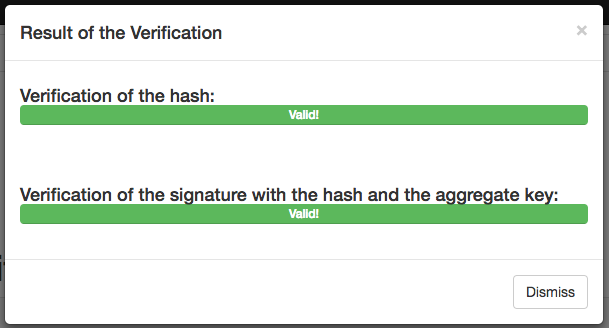
\includegraphics[width=125mm]{modal.jpg}
\caption{Modal box displaying the result of the verifications}
\end{figure}
\leavevmode \\

\section{Conclusion}


%talk about the problem encountered with Linus


% talk about the graphic part at the end
% each 3 seconds

\begingroup
\let\cleardoublepage\clearpage
\bibliographystyle{plainurl}
\bibliography{report}
\endgroup

\end{document}
